\documentclass[10pt]{article}

\usepackage[utf8]{inputenc}

\usepackage{amsmath,amssymb}

\usepackage{esvect}

\usepackage{listings}

\usepackage{color}

\usepackage{graphicx}

\usepackage{float}

\usepackage{blindtext}

\usepackage{tabularx}

\PassOptionsToPackage{hyphens}{url}\usepackage{hyperref}
\hypersetup{
	colorlinks=true,
	linkcolor=blue,
	filecolor=magenta,      
	urlcolor=cyan,
}


\title{Middleware technologies for distributed systems\\Project 4}

\date{2020-2021}



\begin{document}
	\begin{titlepage}
		\begin{figure}[t]
			\centering
\includegraphics[width=0.7\textwidth]{../../docResources/logo_polimi}
		\end{figure}
		\maketitle
		
		\large
		\begin{tabularx}{\linewidth}{@{}lXl@{}}
			\textit{Authors:}  & & \textit{Professors:} \\
			Andrea Falanti      & & Prof.\@ Alessandro Margara\\
			Federico Ferri  & & Prof. Luca Mottola \\
			Abanoub Faltaous & & \\
		\end{tabularx}		
		\thispagestyle{empty}
	\end{titlepage}
	
	\tableofcontents
	\newpage
	
	\section{Introduction}
	\subsection{Description}
	The project consists in a computer simulation, designed to study how virus spread over the population of a certain area. Some individuals are initially infected. If an individual remains close to (at least one) infected individual for more than 10 minutes, it becomes infected. After 10 days, an infected individual recovers and becomes immune. Immune individuals do not become infected and do not infect others. An immune individual becomes susceptible again (i.e., it can be infected) after 3 months.
	
	The simulation area is divided into multiple countries and the program outputs a resume of the country status after each simulation day.
	
	Parameters:
	\begin{itemize}
		\item N = number of individuals
		\item I = number of individuals that are initially infected
		\item W, L = width and length of the rectangular area where individuals move (in meters)
		\item w, l = width and length of each country (in meters)
		\item v = moving speed for an individual
		\item d = maximum spreading distance (in meters): a susceptible individual that remains closer than d to at least one infected individual becomes infected
		\item t = time step (in seconds): the simulation recomputes the position and status (susceptible,infected, immune) of each individual with a temporal granularity of t (simulated) seconds
	\end{itemize}

	\subsection{Additional assumptions} \label{assumptions}
	\begin{itemize}
		\item An individual must be continuously exposed to the virus for 10 minutes to be infected, otherwise the virus has no effect at all (project specifications are a bit vague).
		\item If an individual would go out of the simulation space, it simply inverts its direction.
		\item Parameter v is intended as the max speed possible for an individual, but each individual has a different velocity that is not modified during simulation (text is vague about it).
		\item Each individual position is defined by the input file (Generated randomly).
		\item Each country has same dimensions w,l, if they are not divisors of W and L then the final country of each row / column has as dimensions the remaining space. 
	\end{itemize}
	
	\section{Implementation}
	\subsection{Preface}
	The project is implement in C, using the MPI middleware. MPI allows to parallelize the computation on all the CPU cores, generating potentially a process for each CPU core of the host. This approach exploits better the resources of the system, reducing the time required to perform the simulation, that is really computationally intensive.
	
	The project is composed of multiple C files that can be compiled together using the provided makefile ('make' command), then the program can be launched using the 'mpirun' command.
	
	\subsection{Simulator}
	\subsubsection{MPI initialization}
	As initial step, MPI is initialized and the structs defined in the program that are also used in MPI operations are serialized in a MPI\_Datatype format. Also, a custom MPI\_OP is defined for the country\_report struct, that will be used in a MPI\_Reduce operation explained later in the document. All the processes are part of the default MPI\_COMM\_WORLD communicator. 
	
	MPI usually defines as root processor the processor 0, we followed this convention in our program. The root coordinates the MPI operations and communications between the processes and therefore has a more complex flow compared to other processes.
	
	\subsubsection{Simulator initialization}
	The simulator executable needs as input a txt file with a specific format, which content is used to initialize the simulation parameters. The input file can be generated with the provided utility program (see section \ref{utility}).
	
	\begin{figure}[H]
		\centering
		\makebox[\textwidth][c]{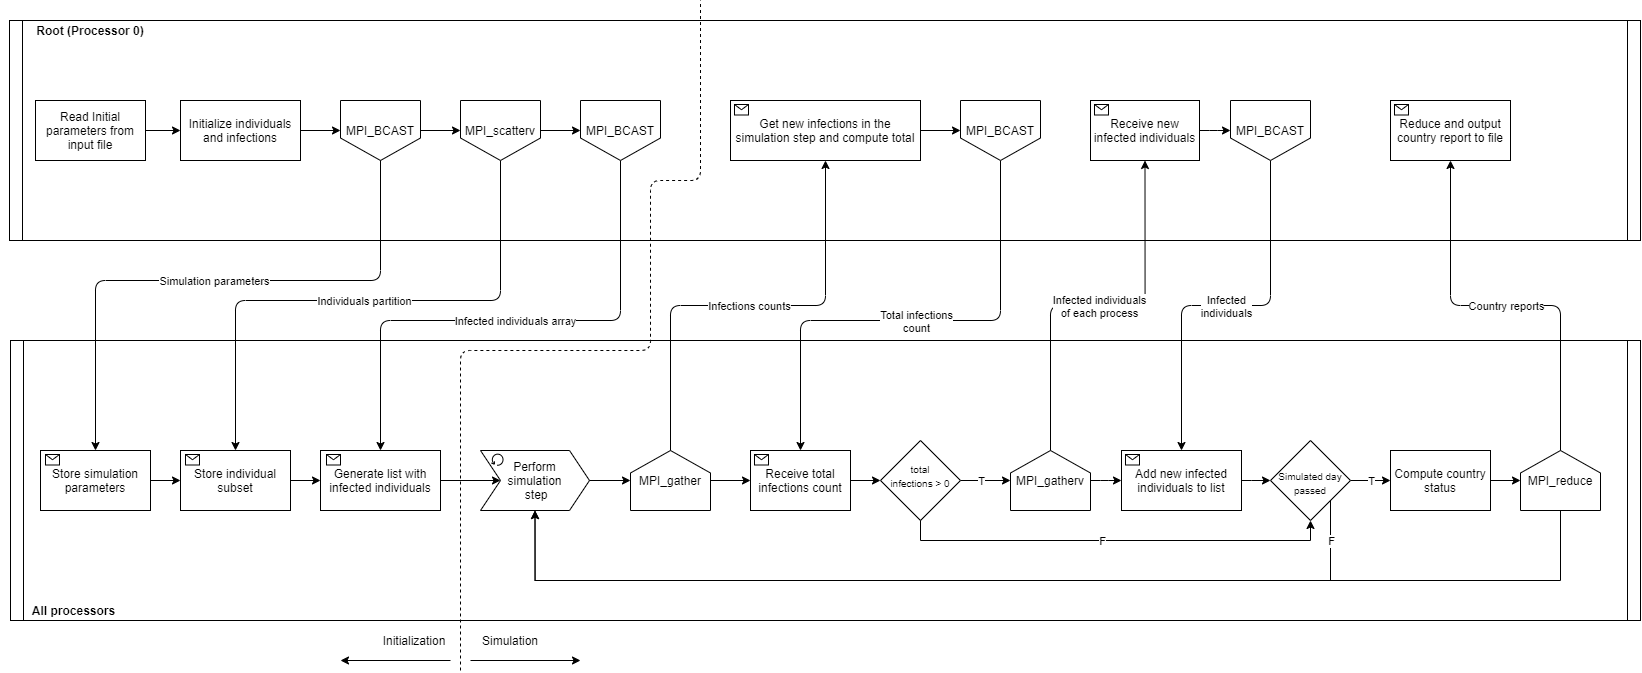
\includegraphics[width=1.5\linewidth]{../../docResources/P4_flow}}
		\caption[]{Program flow}
		\label{fig:p4flow}
	\end{figure}
	
	After MPI initialization, the root reads the input file and initialize all simulation parameters and individuals, then it broadcasts the simulation parameters to all the processes. As next step, the individuals array is scattered among all the processes, each process therefore takes care of a subset of individuals during the simulation, parallelizing the computations required. To check if an individual is near someone infected, all infected individuals position must be known, so the root also broadcast the infected individuals to all the processes.
	
	\subsubsection{Simulation step}
	The root initialize the output file and starts a timer before starting the simulation, the other processes immediately begins. A simulation step consists in multiple operations:
	\begin{itemize}
		\item The status of each individual is updated, in particular a counter of the individual struct is incremented when the individual is infected or immune and after the threshold defined by problem specification is reached then the status is updated and the counter reset (taking care of excess time in the simulation step). If an individual is susceptible, instead, the program checks if an infected individual is nearby (distance $ \le d $): if so, the counter is updated with a mechanism similar to other cases, otherwise it is reset to 0 (see assumptions at section \ref{assumptions}).
		\item The position of each individual is updated.
		\item Status and position of individuals in infected list is updated. Some of them could be already handled in the individuals partition, but are separate entities (no references) so it cause no problems. No stochasticity is involved in the simulation (with given assumptions and simplifications), therefore the infected list will be the same for each process after an update. This avoids to communicate back and fourth the infected individuals at each step.
		\item Returns the total amount of infected individuals in the simulation step, for each process. 
	\end{itemize}

	Then the root gather the infection counters and compute the total: if $ > 0 $ it also gathers the infected individuals and broadcast them to all processes, so that they can add them to the infected list.
	
	When a day pass in the simulation, each process compute the situation in each country, then the root takes all the results with a reduce operation, obtaining the counters for each country when all individuals are considered. The report is printed in an output file.
	
	Simulation steps are repeated until the provided number of days are simulated.
	 
	
	\subsection{Utility program for generating input files} \label{utility}
	A utility program is provided to generate a valid input file for the main program. It accepts 9 command line arguments, in this order:
	\begin{itemize}
		\item N (integer)
		\item I (integer)
		\item W and L (integer)
		\item w and l (integer)
		\item d (float)
		\item t (integer)
		\item maximum speed v (float)
	\end{itemize}

	The output file have all the provided arguments formatted properly and N rows regarding individuals initialization, formatted as {pos.x pos.y v.x v.y}, where the position and velocity are randomly generated in a consistent way with the arguments provided.

	
	\section{Performance analysis}
	The simulation developed has a complexity of $ O(N^2 * sim\_steps) $, given by the interaction check between susceptible individuals and infected ones. Both susceptible and infected counts are always $ \le N $ and the worst cases are when the two counts are actually balanced. Each susceptible individual must check if an infected one is nearby, but if one is found the others are not checked, speeding up the status update.
	
	Using a simulation with these parameters:
	\begin{itemize}
		\item N = 2500
		\item I = 75
		\item 250x250 simulation area, with countries of 50x50
		\item d = 2.03
		\item t = 100
	\end{itemize}
	We performed some tests on the speed of the simulator, simulating 150 days with the same input file, that balance well the infections across the first 40 days, causing major slow downs before proceeding very fast in the remaining days.
	
	The results we obtained are the following:
	\begin{itemize}
		\item 6 processes: 216.117 seconds
		\item 4 processes: 330.496 seconds
		\item 2 processes: 323.427 seconds
		\item 1 process: 237.555 seconds
	\end{itemize}

	Unfortunately, the time of simulations varied a lot even with executions using the same amount of processes. A possible reason of this behavior is the fact that the simulation has been run on a Linux subsystem for Windows, so the fact that it was not the native environment of the machine could have compromised the results.
	Theoretically speaking, we expected to have better results on average by parallelizing across multiple processes, because this allows to check less susceptible individuals per process and so to have a smaller complexity in the 'individual status update' function, which is the bottleneck of the simulator. Of course, communication and coordination costs due to the MPI functions must be heavily considered, because they are done at each simulation step. The slower process limits all the others and the frequent coordination hinders a bit the benefits of running multiple processes, but from the variability of our results is difficult to understand how much the performances actually scale with the number of processes.
	
\end{document}